%Due to the burgeoning interest in web page speed, there has been a recent rise of network caching literature, tools, and companies.
Several papers have analyzed web page performance, the effects of caching, and the relationship between CPU speeds and page load time.
As far as we know, we are the first to jointly isolate all of these factors. % this enables us to easily dissect the effects that caching has on mobile devices.

%\colin{The second and third sentences are too vague.}
\textbf{Web Performance for Desktop}. Related studies~\cite{web-perf-2, web-perf-3} focus on evaluating and optimizing web performance for desktops. Many techniques such as altering content, data compression, proxy services, and CDNs have been exploited to reduce latency for users. These studies focus on high performing end devices such as desktops. We additionally analyzed web performance on a mobile device and show how this differs from classic desktop environments.
%\jamshed{Say something like `the set of assumptions does not hold for mobile.'}

\textbf{Proposed Changes to the Web}. There are many papers~\cite{web-perf-4-new-design, web-caching-4-new-design, web-caching-5-new-design, web-caching-latency-1-new-design, web-caching-latency-2-new-design, web-caching-latency-3-new-design, web-caching-latency-5-new-design, web-caching-latency-6-new-design, web-caching-latency-7-new-design} that propose changes to the web that would improve latency for both desktop and mobile devices through better caching schemes. It is possible that under their proposed changes, caching would have more of a benefit for mobile latency. In this paper, we focus only on today's existing browser infrastructure. % We further show that increasing the hit ratio of caches only provides marginal benefits to mobile page load time.

%\colin{This is very exciting! If there are papers that claim that caching should help mobile latency, we're showing that they're wrong! We need to emphasize this much more!}
\textbf{Web Caching}. Other literature~\cite{web-caching-1, web-caching-2, web-caching-8, web-caching-9} has focused on the benefits of web caching, specifically the reduction of latency for desktops~\cite{web-caching-3, web-caching-4, web-caching-5, web-caching-6, web-caching-7}.
While these papers make note of the several benefits of caching, their set of assumptions do not necessarily hold for mobile devices, which have significantly less computational power. 

\textbf{WProf}. Wang et al.~\cite{wang2013demystifying} is perhaps the closest research to ours. WProf found that the fraction of bytes cached in a web page is not proportional to the reduction in page load time. By dissecting the process of loading a page, they found that the cached objects are typically not on the critical path, and thus do not reduce the user's overall latency. 

WProf focuses on devices with rich computational resources rather than the more common mobile devices. Our results on mobile are consistent with WProf's desktop counterpart. In fact, the results we present show that caching has even smaller benefits on mobile devices.
% Good.

\textbf{Mobile, CPU Speeds, and PLT}.
Some research has also investigated the extent to which CPU speed determines page load time, for desktop~\cite{CPU-plt-1} and mobile devices~\cite{CPU-plt-2, CPU-plt-3}.
%Research has also been conducted regarding the correlation between CPU speed and page load times. Jones et al. ~\cite{CPU-plt-1} noted that increased page load time on mobile devices was due to the lack of CPU power, but did not provide backing evidence.
Wang et al.~\cite{CPU-plt-2, CPU-plt-3} have determined that the largest delay factor in desktop web page loading is object rendering in the browser. They went further to show that CPU constraints are the lead cause of slow resource loading. 
With a large data set, we bolster the claim that suggests that CPU constraints are the critical factor in determining page load time. We also demonstrate that web caching has diminishing benefits due to the limited CPU speeds of mobile devices.
%\jamshed{TODO: discuss other methodologies, why is our apparatus novel?}
% \jamshed{From Colin: Most other papers measure results "in the wild", i.e. on real networks. That's useful for the final results, but it's hard to control it well enough to get repeatable results.}
%\begin{figure}[t]
%    %\hspace{-10pt}
%    \figuretitle{Fraction Reduction in PLT with Inflated Delays}
%    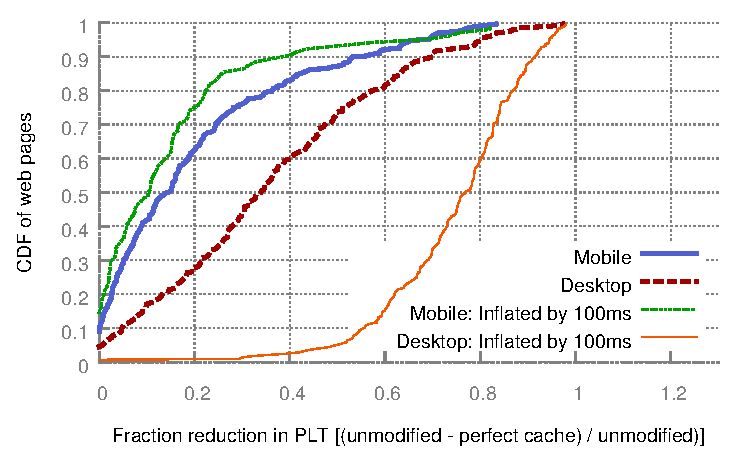
\includegraphics[width=3in]{../graphs/percent_plt_reduction/percent_reduction_linear_inflated.pdf}
%    \caption[]{\label{fig:inflated_delays}In networks with high latency, caching has a negligible effect on mobile PLTs, but a significant benefit for desktop PLTs.}
    % Just remove the first sentence of the caption?
%\end{figure}
\begin{figure}[t]
    %\hspace{-10pt}
    \figuretitle{Page Load Time}
    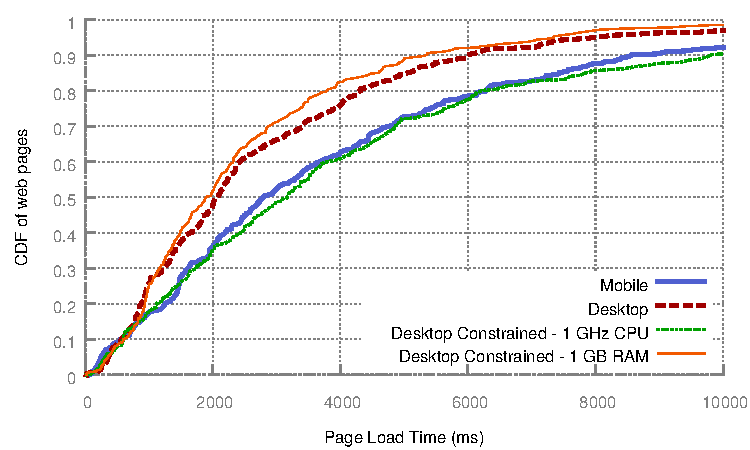
\includegraphics[width=3in]{../graphs/plt_comparison/plt_differences.pdf}
    \caption[]{\label{fig:plt_differences}Web pages take longer to load on devices constrained with CPU speeds.}
\end{figure}